\documentclass[twocolumn]{article}
\usepackage[letterpaper, left=2.5cm, right=2.5cm, top=2.5cm, bottom=2.5cm]{geometry}
\usepackage{graphicx}
%\usepackage{estopdf}
\usepackage{verbatim}
\usepackage{listings}
\begin{document}

\lstset{
language=C,                             % Code langugage
basicstyle=\ttfamily,                   % Code font, Examples: \footnotesize, \ttfamily
numbers=left,                           % Line nums position
numberstyle=\tiny,                      % Line-numbers fonts
stepnumber=1,                           % Step between two line-numbers
numbersep=5pt,                          % How far are line-numbers from code
frame=none,                             % A frame around the code
tabsize=2,                              % Default tab size
captionpos=b,                           % Caption-position = bottom
breaklines=true,                        % Automatic line breaking?
breakatwhitespace=false,                % Automatic breaks only at whitespace?
showspaces=false,                       % Dont make spaces visible
showtabs=false,                         % Dont make tabls visible
columns=flexible                        % Column format
}

\title{CMPUT 313 Assignment 2}
\date{Tuesday, March 13}
\author{Stephen Jahns and Marek Kundera}

\maketitle

\section*{Introduction}

	Choosing an appropriate backoff strategy for the Slotted ALOHA MAC layer
	protocol depends on a series of factors. In this report, we have
	simulated the Probabilistic Backoff ($P$), Interval-Based Backoff ($I$),
	and Truncated Binary Exponential Backoff ($B$) strategies. In addition,
	we have simulated the Time Division Multiplexing ($T$) protocol for
	additional comparison. Our simulation was based on several assumptions
	found in the problem specification and on a terse description of each
	protocol:

$T$: a station $i$ only transmits at slot number $mN + i$, $m$ = 0, 1, 2, ...
$N$, where $m$ is the cycle number, and $N$ is the number of stations

$P$: a station will try to transmit immediately on generation, or retransmit
with $1/N$ probability at each subsequent slot

$I$: a station will try to transmit immediately on generation, or retransmit at
a slot 1 to $N$ slots later, chosen randomly

$B$: a station will try to transmit immediately on generation, or retransmit at
a slot 1 to 2 slots later, then 1 to 4 slots later, or eventually 1 to $2^i$
slots later, chosen randomly until the frame successfully transmits

	To set some groundwork, we will begin by outlining our expectations with
	a preliminary analysis. Next we will briefly explain the main
	functionality and design of our \verb|psim| simulator. Then we will reveal the
	simulation results with the help of some tables and graphs, paired with
	the parameters we used to generate the media. Finally, we will examine
	each protocol's performance by analyzing their average throughputs and
	the overall average per-frame slot time delays of the successfully
	transmitted frames. In addition, we will examine the fairness of each
	protocol by observing the number of undelivered frames under each
	protocol at the individual stations.

\subsection*{Time Division Multiplexing} Here we expect that as the probability
of frame generation, $p$, increases, the average frame delay should increase. This is
because in any given cycle of $N$ slots, the probability of a frame being
generated at that slot increases. Therefore as $p$ increases, up to $N$ frames
might be generated in a cycle.  On the other hand, the mean throughput should
increase in direct proportion to $p$. As $p$ increases, it is more likely frames
will be available for transmission in a given cycle. In other words, it is more
likely a station will not waste its designated slot time. Furthermore, since
each station has a designated slot only it can transmit on, it is not possible
for collisions to occur between the stations. 
A potential serious weakness of TDM is that if the load is not equally balanced 
between the stations on the bus, unnecessary delays may occur, especially if only
a single station has a very large number of frames queued for a period of many slots.
The busy station will experience delays of $N$ slots between each frame transmitted,
while all other slots are left unused, leaving the overall hub throughput very low and
the delay unnecessarily high.

\subsection*{Probabilistic Backoff} Notice that for a probability of successful
transmission of $1/N$, we need $N$ stations to each have a frame queued for
transmission, in order for one to \emph{likely} transmit. We can build on this
observation and hypothesize that at some $p$, every station will be generating
frames faster than it can transmit them. And therefore, the throughput will
level off in concert with the probability that \emph{exactly one} station
transmits, i.e. let event $ExactlyOneTx$ represent the case where exactly one
station is transmitting. Thus, when $N$=20 stations, $Prob(ExactlyOneTx)$ =
$C(20,1)\times(1/20)\times(19/20)^{19}$ = 0.377. For 20 stations, it is likely
then that when $p=0.377/20=0.019$, we can expect the throughput to begin
leveling off and for the average frame delay to start increasing. This is
because as $p$ increases, frames are more likely to generate, while the
throughput remains the same. And so, the queue can only get larger thus each
frame must wait longer before moving to the front of the queue for transmission.

\subsection*{Interval-Based Backoff} In a similar fashion to the probabilistic
backoff, as $p$ is increased, we predict that some critical point will be reached
where the rate of generation will be higher than the rate of transmission, and so the
queues at each station will grow, increasing the average frame delay. Additionally,
the throughput will level out as the probability of a collision stabilizes along with
the rate of successful transmission. Consider an analogy of $N$=20 buckets. At each time
slot, each station has $p$ chance of adding a 'ball to one bucket'. Therefore, in the
long run, the frames generated per slot is $N\times p$ while the rate of transmission
can be 1 at best, but realistically much lower (let's say $Z$). It is easy to see that
as $p$ increases, eventually the rate of generation will be greater than the rate of
transmission (or throughput), i.e. $N\times p \geq Z$. $Z$ can be said to be equal to
the probability that a bucket has exactly one ball. This isn't the same probability as
above, and it won't be calculated as it would involve higher level probabilistic math.
At this point however, the throughput will will level out and the average frame delay will increase
as $p$ increases.

\subsection*{Truncated Binary Exponential Backoff}

Truncated binary exponential backoff is more or less a fancy version of interval backoff 
where instead of a fixed interval size of $N$ slots to randomly backoff for, the interval
starts at 4 slots and doubles at every collision until 1024. Due to this property, if a
single station has at least 9 consecutive transmission attempts with collision, 
the interval before the next transmission attempt could be as long as 1024 slots. During low
loads on the bus, we should expect small delays as immediate transmission of a frame upon 
generation (if the transmission queue was previously empty) or after a successful transmission
is allowed. During progressively higher loads, the relative performance between TBEB and IB and PB in
in terms of hub throughput and average delivery delay may be difficult to predict. 

\section*{Methods}

The \verb|psim| simulator was implemented in C++. It requires several parameters
at the command line:

\begin{center}\verb|psim Protocol N p R T seed1 seed2 ... seedT|\end{center}

 \verb|Protocol| can taken on a value of \verb|T|, \verb|P|, \verb|I|, or \verb|B|, depending on
what protocol is being simulated. The parameter \verb|N| represents the number of
stations that will be transmitting under the protocol. \verb|p| represents the
probability that a frame will be generated at each station. \verb|R| represents the
number of slots that the experiment will run, and is therefore the time-measure
for the experiment. And \verb|T| represents the number of trials the simulation will
run, while the following \verb|seed1...seedT| inputs are used to reseed the
randomization functions for each trial. 

For the purpose of this simulation, the
values \verb|N=20|, \verb|R=50000|, and \verb|T=5| will be fixed. In other words, we will
simulate 5 trials where 20 stations transmit over a time period of 50,000 slots.
The observations shown later are based on 5 trials that were seeded with values
1, 2, 3, 4, 5, respectively.

\verb|psim| functions by simulating \verb|T| independent trials of hub of
\verb|N| stations running for \verb|R| time slots, using the random number
generator seeds separately specified for each trial. At the beginning of each
timeslot, each station generates a new frame on its transmission queue with
probability \verb|p|. Then, the delay value in time slots is incremented for
each frame on each stations transmission queue.  Then, the simulator determines
which and how many stations will attempt transmission in that timeslot,
according to the MAC protocol specified in \verb|Protocol|. If there is only one
station attempting transmission, the transmission is deemed successful and the
frame is removed from that station's queue. If there are more than one
transmissions, a \verb|tx_collide(slot)| method is executed on each station that
partly implements the station's backoff protocol as specified in
\verb|Protocol|.

The simulator outputs the parameters (minus the seeds) on the first line. After
running all trials, it calculates and prints 95\% confidence intervals for the
overall average throughput in frames delivered per time slot, and delay in slots
for each frame successfully delivered, on lines 2 and 3 respectively. Delay was 
calculated from the time of frame generation to the time of successful delivery in slots,
in a matter that the minimum delay is 1 if the frame is generated in the same slot that it is
delivered in. Confidence
intervals were calculated using appropriate t-statistics for the number of
trials from a file labelled \verb|tvalues.dat|. Per-station statistics were output
on the remaining lines, where each line started with \verb|nN|, the id of the station,
followed by confidence intervals for throughput and delay per frame delivered, and finally
the ratio of undelivered frames to total frames generated by that station for each trial 
separately, all on the same line.

Experiments were automated using the BASH script \verb|make_plot.sh| 
to run the simulator for each protocol over ranges of \verb|p| values ranging
from 0.00 up to 0.04. The scripts parsed data from the output into appropriately
formatted data files that were sent to GNUPLOT for plotting.

\section*{Results}

\begin{figure}
    \centering \includegraphics[width=8cm]{plots/delay_big.eps}
    \caption{\footnotesize  Average delay per frame under each protocol for
    $p$:(0,0.04; @0.005 increments). Used to illustrate what happens as $p$
    nears 0.04.} \label{fig:delay_big}
\end{figure}

\begin{figure}
    \centering \includegraphics[width=8cm]{plots/throughput_big.eps}
    \caption{\footnotesize Mean throughput of all stations under each protocol
    for $p$:(0,0.04; @0.005 increments). Used to illustrate what happens as $p$
    nears 0.04.} \label{fig:throughput_big}
\end{figure}

\begin{figure}
    \centering \includegraphics[width=8cm]{plots/small_delay.eps}
    \caption{\footnotesize Average delay per frame under each protocol for
    $p$:(0,0.015; @0.001 increments). Used to illustrate what happens as $p$
    nears 0.} \label{fig:delay_small}
\end{figure}

\begin{figure}
    \centering \includegraphics[width=8cm]{plots/small_throughput.eps}
    \caption{\footnotesize Mean throughput of all stations under each protocol
    for $p$:(0,0.015; @0.001 increments). Used to illustrate what happens as $p$
    nears 0.} \label{fig:throughput_small}
\end{figure}

\begin{figure}
    \centering \includegraphics[width=8cm]{plots/ib_diverge_delay.eps}
    \caption{\footnotesize Average delay per frame under each protocol for
    $p$:(0,0.02; @0.001 increments). Used to illustrate where protocols begin to
    diverge significantly. Especially, protocol $I$ at $p$=0.015.}
    \label{fig:delay_ib}
\end{figure}

\begin{figure}
    \centering \includegraphics[width=8cm]{plots/ib_diverge_throughput.eps}
    \caption{\footnotesize Mean throughput of all stations under each protocol
    for $p$:(0,0.02; @0.001 increments). Used to illustrate where protocols
    begin to diverge significantly. Especially, protocol $I$ at $p$=0.016.}
    \label{fig:throughput_ib}
\end{figure}

\begin{figure}
    \centering \includegraphics[width=8cm]{plots/tpbi_delay.eps}
    \caption{\footnotesize Average delay per frame under each protocol for
    $p$:(0.01,0.021; @0.001 increments). Used to illustrate the points where the
    protocols intersect.} \label{fig:delay_diverging}
\end{figure}

\begin{figure}
    \centering \includegraphics[width=8cm]{plots/tpbi_throughput.eps}
    \caption{\footnotesize Mean throughput of all stations under each protocol
    for $p$:(0.01,0.021; @0.001 increments). Used to illustrate the points where
    the throughput for protocols $I$ and $P$ begins to level off.}
    \label{fig:throughput_diverging}
\end{figure}


For ranges of frame generation probabilities per station per slot ranging
from 0.0 to 0.04, plots of average delay in slots per frame successfully delivered and
of throughput in number of frames per timeslot were obtained. 

In Figure~\ref{fig:delay_big}, we see that over larger values of $p$ ranging up to
0.04, there is a clear separation in delay levels for each protocol. Interval backoff
produces the largest delays, followed by probabilistic backoff. Truncated binary exponential
backoff produces the least delays of the Slotted ALOHA MAC protocols. Time division multiplexing,
however, provides delivery delays at $p=0.04$ that are a tiny fraction of the delays of the 
ALOHA protocols. Similar results exist for throughput at higher loads ($p$ approaching 0.04) as 
seen in Figure~\ref{fig:throughput_big}. TBEB provides the highest throughput at high load,
followed by IB and PB. TDM provides a higher throughput at high load than the ALOHA protocols,
but by a much smaller margin (~10\% higher than TBEB) than exhibited by the difference in
delays.

At smaller loads (approx. $p<0.013$), the frame delivery delays for TDM become
larger than that of the ALOHA protocols (Figure~\ref{fig:delay_small}). The relative delays 
between the different ALOHA protocols also changes. For $p<0.012$, TBEB has the smallest delay,
but the delay increases strongly above that value. Interval backoff has the smallest delays
for 
$p \in (0.012, 0.016)$, after which the delay for IB jumps up sharply (Figure~\ref{fig:delay_ib}).
For $p > 0.016$, TDM has less delay than any of the ALOHA protocols, and PB has the smallest 
delay of the ALOHA protocols for $p \in (0.016, 0.02)$, after which the delay jumps to above
that of TBEB (Figure~\ref{fig:delay_diverging}). TBEB has the least delay of the ALOHA protocols
for $p > 0.02$.

All protocols produce very similar throughputs at low load for $p \in (0, 0.016)$
(see Figures ~\ref{fig:throughput_small} and ~\ref{fig:throughput_ib}), where
all throughputs appear to increase linearly with frame generation probability. 
Above $p=0.016$, IB throughput drops fairly quickly by about 20\% and flattens to a throughput
of about 25\% for all higher loads. Above $p=0.02$, PB throughput drops a little and flattens
to about 40\% for all higher loads. 

\begin{figure}
    \centering 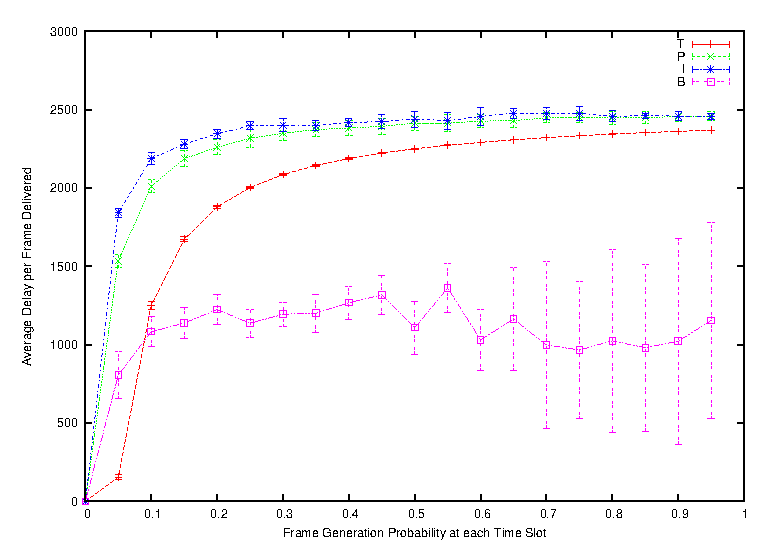
\includegraphics[width=8cm]{plots/fullrange_delay5000.eps}
    \caption{Average delay per frame delivered on hub for full range of per
    slot, per station frame generation probability, tested for each MAC
    protocol  $R=5000$ slots, $T = 5$ trials.}
    \label{fig:fullrange_delay}
\end{figure}

\begin{figure}
    \centering \includegraphics[width=8cm]{plots/fullrange_throughput5000.eps}
    \caption{Average throughput on hub for full range of per
    slot, per station frame generation probability, tested for each MAC
    protocol  $R=5000$ slots, $T = 5$ trials } 
    \label{fig:fullrange_throughput}
\end{figure}

\begin{table*}
    \centering 
%B 20 0.040000 50000 5 1 2 3 4 5
    \label{fig:fairness_tdm}
    \begin{tabular}{l|c|c|c|c|c}
           & 1 & 2 & 3 & 4 & 5 \\
        \hline
        n1 & 0.006471 & 0.000503 & 0.000989 & 0.000505 & 0.001422 \\
        n2 & 0.000987 & 0.002000 & 0.002017 & 0.002999 & 0.001004 \\
        n3 & 0.000501 & 0.001001 & 0.000988 & 0.001035 & 0.000000 \\
        n4 & 0.000000 & 0.000501 & 0.000985 & 0.000481 & 0.000000 \\
        n5 & 0.000000 & 0.000489 & 0.000985 & 0.000986 & 0.000000 \\
        n6 & 0.000000 & 0.000517 & 0.000000 & 0.000000 & 0.001496 \\
        n7 & 0.002455 & 0.002026 & 0.000000 & 0.001485 & 0.000484 \\
        n8 & 0.001047 & 0.000000 & 0.000000 & 0.000000 & 0.002499 \\
        n9 & 0.000000 & 0.000000 & 0.002534 & 0.003348 & 0.000000 \\
       n10 & 0.000000 & 0.001004 & 0.000991 & 0.000000 & 0.001492 \\
       n11 & 0.000000 & 0.000495 & 0.003854 & 0.001487 & 0.001453 \\
       n12 & 0.001505 & 0.001004 & 0.002004 & 0.001037 & 0.000000 \\
       n13 & 0.002463 & 0.000000 & 0.003085 & 0.000000 & 0.000513 \\
       n14 & 0.002552 & 0.001035 & 0.000503 & 0.004805 & 0.003038 \\
       n15 & 0.002014 & 0.000000 & 0.001000 & 0.000490 & 0.002535 \\
       n16 & 0.000000 & 0.000496 & 0.001001 & 0.000506 & 0.000000 \\
       n17 & 0.000000 & 0.000514 & 0.004460 & 0.001044 & 0.000978 \\
       n18 & 0.000000 & 0.000499 & 0.001999 & 0.000000 & 0.000512 \\
       n19 & 0.000000 & 0.003044 & 0.000986 & 0.000000 & 0.002092 \\
       n20 & 0.000501 & 0.000507 & 0.000000 & 0.000494 & 0.000504

    \end{tabular}
%B 20 0.040000 50000 5 1 2 3 4 5
%0.696424 0.691729 0.701119
%4558.648255 4053.037562 5064.258947
    \caption{ Ratios of undelivered to total generated frames, per station, per trial using
        time division multiplexing, $p=0.04$, $R=50000$ slots, $T = 5$ trials.  
        Each column corresponds to a single trial, each row corresponds to a single station. }

\end{table*}

\begin{table*}
    \centering 
%B 20 0.040000 50000 5 1 2 3 4 5
    \label{fig:fairness_pb}
    \begin{tabular}{l|c|c|c|c|c}
           & 1 & 2 & 3 & 4 & 5 \\
        \hline
        n1 & 0.508249 & 0.581281 & 0.539540  & 0.536810 & 0.536203 \\
        n2 & 0.519899 & 0.544526 & 0.561975  & 0.563332 & 0.536524 \\
        n3 & 0.481934 & 0.525169 & 0.486970  & 0.501256 & 0.544828 \\
        n4 & 0.545960 & 0.516467 & 0.479901  & 0.471414 & 0.493199 \\
        n5 & 0.566901 & 0.565152 & 0.511707  & 0.531282 & 0.539249 \\
        n6 & 0.535802 & 0.483191 & 0.508449  & 0.525551 & 0.479410 \\
        n7 & 0.545680 & 0.511827 & 0.541955  & 0.522461 & 0.505500 \\
        n8 & 0.533605 & 0.493834 & 0.534942  & 0.541357 & 0.506216 \\
        n9 & 0.530633 & 0.490852 & 0.550930  & 0.542089 & 0.502367 \\
       n10 & 0.559280 & 0.528793 & 0.560729  & 0.510886 & 0.522739 \\
       n11 & 0.518182 & 0.546937 & 0.552566  & 0.542323 & 0.528358 \\
       n12 & 0.518127 & 0.529263 & 0.535873  & 0.511548 & 0.521608 \\
       n13 & 0.472489 & 0.473892 & 0.547284  & 0.516274 & 0.522795 \\
       n14 & 0.499205 & 0.546417 & 0.497184  & 0.520791 & 0.538313 \\
       n15 & 0.545084 & 0.524158 & 0.527061  & 0.527906 & 0.573762 \\
       n16 & 0.503090 & 0.526585 & 0.511013  & 0.571001 & 0.580835 \\
       n17 & 0.519297 & 0.563939 & 0.516014  & 0.499746 & 0.511922 \\
       n18 & 0.508870 & 0.549527 & 0.542843  & 0.530334 & 0.513667 \\
       n19 & 0.545858 & 0.515464 & 0.560582  & 0.538499 & 0.518900 \\
       n20 & 0.495988 & 0.556727 & 0.498999  & 0.507109 & 0.526804
    \end{tabular}
%B 20 0.040000 50000 5 1 2 3 4 5
%0.696424 0.691729 0.701119
%4558.648255 4053.037562 5064.258947
    \caption{ Ratios of undelivered to total generated frames, per station, per trial using
       probabilistic backoff, $p=0.04$, $R=50000$ slots, $T = 5$ trials.
    Each column corresponds to a single trial, each row corresponds to a single station. }

\end{table*}

\begin{table*}
    \centering 
%B 20 0.040000 50000 5 1 2 3 4 5
    \label{fig:fairness_ib}
    \begin{tabular}{l|c|c|c|c|c}
           & 1 & 2 & 3 & 4 & 5 \\
        \hline

        n1 & 0.682902 & 0.686082 & 0.700204 & 0.690148 & 0.673203 \\
        n2 & 0.679692 & 0.689398 & 0.697190 & 0.661972 & 0.675635 \\
        n3 & 0.716981 & 0.682341 & 0.659226 & 0.673226 & 0.666492 \\
        n4 & 0.713648 & 0.716935 & 0.692615 & 0.673288 & 0.685700 \\
        n5 & 0.677587 & 0.694077 & 0.702149 & 0.672148 & 0.694153 \\
        n6 & 0.688391 & 0.706201 & 0.702863 & 0.679980 & 0.655243 \\
        n7 & 0.658811 & 0.664447 & 0.666136 & 0.721930 & 0.687562 \\
        n8 & 0.671120 & 0.683063 & 0.664175 & 0.705179 & 0.707486 \\
        n9 & 0.691258 & 0.666667 & 0.675761 & 0.691448 & 0.709483 \\
       n10 & 0.691358 & 0.669888 & 0.666159 & 0.695152 & 0.701021 \\
       n11 & 0.686657 & 0.681751 & 0.690379 & 0.676530 & 0.679303 \\
       n12 & 0.689154 & 0.651744 & 0.681750 & 0.700640 & 0.704902 \\
       n13 & 0.715681 & 0.692882 & 0.686462 & 0.690809 & 0.677016 \\
       n14 & 0.680972 & 0.706897 & 0.681089 & 0.699294 & 0.698234 \\
       n15 & 0.686216 & 0.662398 & 0.699356 & 0.691370 & 0.658612 \\
       n16 & 0.682927 & 0.714427 & 0.695309 & 0.712512 & 0.700500 \\
       n17 & 0.647456 & 0.703210 & 0.685269 & 0.705513 & 0.722195 \\
       n18 & 0.670229 & 0.667469 & 0.682620 & 0.694542 & 0.698836 \\
       n19 & 0.698437 & 0.688623 & 0.689368 & 0.699150 & 0.673657 \\
       n20 & 0.672286 & 0.701729 & 0.689209 & 0.674254 & 0.662021


    \end{tabular}
%B 20 0.040000 50000 5 1 2 3 4 5
%0.696424 0.691729 0.701119
%4558.648255 4053.037562 5064.258947
    \caption{ Ratios of undelivered to total generated frames, per station, per trial using
        interval backoff, $p=0.04$, $R=50000$ slots, $T = 5$ trials.  
        Each column corresponds to a single trial, each row corresponds to a single station. }

\end{table*}

\begin{table*}
    \centering 
%B 20 0.040000 50000 5 1 2 3 4 5
    \label{fig:fairness_tbeb}
    \begin{tabular}{l|c|c|c|c|c}
           & 1 & 2 & 3 & 4 & 5 \\
        \hline
n1 & 0.077351 & 0.118118 & 0.425962 & 0.002500 & 0.052495 \\
n2 & 0.125247 & 0.062253 & 0.008973 & 0.386563 & 0.084267 \\
n3 & 0.061347 & 0.106634 & 0.146091 & 0.035376 & 0.079079 \\
n4 & 0.053150 & 0.073552 & 0.000000 & 0.316767 & 0.063099 \\
n5 & 0.115442 & 0.031403 & 0.084800 & 0.093294 & 0.018945 \\
n6 & 0.290680 & 0.310675 & 0.084221 & 0.040675 & 0.016035 \\
n7 & 0.285861 & 0.006979 & 0.057115 & 0.171313 & 0.364198 \\
n8 & 0.143426 & 0.054381 & 0.311475 & 0.043000 & 0.161356 \\
n9 & 0.016907 & 0.008755 & 0.156189 & 0.109576 & 0.201082 \\
n10 & 0.043048 & 0.133580 & 0.099445 & 0.224008 & 0.052000 \\
n11 & 0.090303 & 0.126420 & 0.418695 & 0.242541 & 0.003605 \\
n12 & 0.080145 & 0.000000 & 0.000000 & 0.339708 & 0.086697 \\
n13 & 0.185393 & 0.203203 & 0.003885 & 0.103681 & 0.031915 \\
n14 & 0.049010 & 0.190793 & 0.000000 & 0.144299 & 0.212091 \\
n15 & 0.240223 & 0.082819 & 0.314556 & 0.121367 & 0.091960 \\
n16 & 0.150581 & 0.078744 & 0.427317 & 0.024150 & 0.287167 \\
n17 & 0.016312 & 0.204412 & 0.003458 & 0.018482 & 0.377398 \\
n18 & 0.119456 & 0.179462 & 0.059233 & 0.029340 & 0.068982 \\
n19 & 0.135551 & 0.203085 & 0.072709 & 0.002467 & 0.083416 \\
n20 & 0.118554 & 0.331832 & 0.097561 & 0.129732 & 0.238192 
    \end{tabular}
%B 20 0.040000 50000 5 1 2 3 4 5
%0.696424 0.691729 0.701119
%4558.648255 4053.037562 5064.258947
    \caption{ Ratios of undelivered to total generated frames, per station, per trial using
        truncated binary exponential backoff, $p=0.04$, $R=50000$ slots, $T = 5$ trials.  
        Each column corresponds to a single trial, each row corresponds to a single station. }

\end{table*}

For the range of $p$ values that could be tested using \verb|R=50000| (higher
$p$ values resulted in at least polynomially higher simulation run times as the frame queues
became heavier loaded), we did not see a point where TBEB throughput levels off. Running
the simulator under the same conditions as before but with \verb|R=1000| and \verb|p| ranging
from 0 to 1, TBEB throughput appears to increase steadily until about 78\% at about $p = 0.5$,
and the same plot for \verb|R=5000| shows TBEB throughput leveling off at about 93\% 
(Figure~\ref{fig:fullrange_delay}). At \verb|R=5000|, IB and PB delays appear to level off at the
same values as for \verb|R=50000|.

In Figure~\ref{fig:fullrange_delay}, we also see that with sufficiently high load, TBEB yields
a lower average delay than T

In order to determine the relative fairness of each protocol with respect to individual stations
competing for transmissions on the hub, we measured per trial, per station ratios of 
undelivered frames to total frames generated at that station. For this metric, if the ratio
is 0 at the end of the trial, all frames were successfully delivered, and if the ratio is 1, 0
frames were successfully delivered. Simulations were run for
each of the protocols, and results 
backoff protocols are listed in Tables 1 - 4 . In Table 1, the ratios do not grow much larger 
than one for any station on any trial, meaning that all stations were able to transmit
nearly all their frames by the end of the trial. In Table 2, for PB we see that the
ratios for each station never stray below 0.45 or above 0.6 within a trial. Table 3 shows
similar results for interval backoff. In Table 4,
within a single trial, the ratios for each station range from 0 (all generated frames 
successfully delivered) to 0.43 (nearly half of all frames unsuccessfully delivered, left
in queue at end of trial).



\section*{Discussion}
Our comparison of the protocols will be based on 3 metrics: delay, throughput, and fairness.

\subsection*{Delay} To effectively compare the protocols on the delay metric, we have generated
graphs for different ranges of $p$. We will compare the protocols at these ranges.

\emph{range: 0,0.015} Figure 3

$T$ performs the worst until $p$=0.013, where both $P$ and $B$ intersect with it and start performing worse.

This occurs because the few frames that are generated on the $T$ protocol have to wait to transmit on a valid slot,
while perfectly valid slots are available but not used. On average we would expect a frame to have to wait $N/2 = 20/2 = 10$
slots before transmitting, when the queued frames at each station are small or nonexistent. At $p$=0.013, protocols $P$
and $B$ intersect with $I$, because their average frame delay exceeds a value of 10. This is a result of collisions
that are inevitable for these protocols. As a result of the collisions, the time delay has risen polynomially. In contrast,
the $T$ protocol does not experience collisions, and so the time delay is growing linearly.

$P$ performs second worst until $p$=0.013, where $B$ starts performing the worst

This means that at this point, there are more collisions occuring under the $B$ protocol and increasing the
observed time delay. This occurs because the backoff interval for $B$, i.e. 2^{collisions} is smaller than under $P$, i.e. N slots when collisions do not
occur too often (because frame generation is low).

$I$ and $B$ perform similarly until $p$=0.012, where $B$ deviates off; at this point $I$ becomes the 
best performer.

Same reason as above, more collisions are occuring under $B$ than under $I$, bumping up the time delay. Again because
the backoff interval depends on collisions and few collisions have occured, such that $2^{collisions} < N$.

\emph{range: 0.01,0.021} Figure 7

$T$ performs the best after $p$=0.016, when $I$ deviates significantly

Since no collisions occur under $T$, the delay continues to rise linearly and is outperforming all the other
protocols. $I$ has deviated significantly because at around $p$=0.016 it reached a critical point predicted at
in our Introduction. As $p$ increases, eventually the rate of frame generation will be greater than the rate of
transmission (or throughput), i.e. $N\times p \geq$ the rate of transmission. At this point we see in 
Figure 2 that the throughput has reached a maximum of around 0.3 and begun to decrease. In turn the average frame
delay should increase as $p$ grows larger.

$I$ intersects with $B$ shortly after $p$=0.016 and becomes the worst performer

There are more collisions occuring under $I$ at this point than under $B$, because $B$ now has 'evolved' a larger
backoff interval. So while frames continue to be transmitted successfully under $B$, the frames are often
colliding under $I$ and therefore waiting longer in the station queue. Under $I$ we see that the throughput starts to decrease
as more slots are wasted because nothing is successfully transmitted over them.

$P$ intersects with $B$ at $p$=0.02 and becomes the second worst performer

This observation occurs for the same reason as that seen for $I$ and $B$ above. Only $P$ appears to be performing better than
$I$. This is because the frames under $P$ attempt to transmit on each subsequent slot. Therefore, statistically speaking, a frame's
chance of transmitting increases each time by a factor of $1/N$ such that by the $N^{th}$ attempt it has likely tried to
retransmit at least once. In contrast, under $I$ it will \emph{at most} try to transmit $N$ times in a cycle. And at worst, it might only
attempt to retransmit once in a cycle. So naturally it would make sense that $P$ is performing better than $I$.

\emph{range: 0,0.04} Figure 1
$T$ performs the best as $p$ approaches 0.04
$B$ performs second best
$P$ performs third best
$I$ performs worst
i.e. these are trends that manifested and continue from figure 7; no discussion necessary.

\emph{range: 0,1} Figure 9
$T$ performs best until $p$=0.1 where it intersects with $B$ and performs second best after the fact
$B$ performs best from $p$ \geq 0.1

Notice in Figure 9 that at $p$=0.05, the delay for $T$ increases significantly. This is because
$p$ = 0.05 is equal to $1/N = 1/20 = 0.05$. At this point the chance of frame generation is equal to the
rate of transmission and the queues at each station are growing. Notice on Figure 10 that by
$p$ = 0.1 the throughput for $T$ has maximized at 1, i.e. a frame is transmitted by one station at every slot.

$T$ and $B$ appear to intersect at a frame delay around 1000. This is because the delay for $B$ levels out around $2^{10} = 1024$.
It seems then that a backoff interval of 1024 slots is sufficient for $N$=20 stations. It is worth noting the
range of the confidence interval. This is seen because some frames see an empty slot and transmit immediately while
other frames might wait a very long time before transmitting, even though slots are available.

$P$ continues to perform 3rd best until about $p$=0.9, where its performance converges with that of $I$
$I$ performed the worst for the vast majority of this range

Protocol $P$'s better performance than $I$ was explained earlier. 

\subsection*{Throughput}

\subsection*{Fairness} 

In our simulation, the rate of frame generation for each station is equal, so there is
equal demand for the channel from all stations. Therefore, a fair MAC protocol should provide
approximately equal access to each station over the course of a single trial (if a trial is
sufficiently long). In order to quantify this, we recorded the ratio of undelivered frames
to total generated frames for each station for each trial run by the simulator. If each station
is given fair access to the channel, these ratios should be approximately for each station. For
time division multiplexing, probabilistic backoff, and interval backoff, this is what we 
observed (Table 1).

Time division multiplexing is by its definition clearly a fair protocol, as each station is 
granted exactly equal access to the channel in the form of its unique assigned slot. No 
collisions are possible. This assertion is backed up by our observation in Table 1 that 
all stations were able to transmit nearly all their frames by the end of each trial. The 
stations that did not transmit all of them likely had generated the frames soon before the 
end and had not yet had time to empty their queue.

Probabilistic backoff was also observed to be a fair protocol, in Table 2 we see all the 
ratios hovering in a reasonably small interval between 0.45 and 0.6, meaning that all stations
were able to successfully transmit approximately half their generated frames by the end of each
trial. The fairness in PB is due how the backoff procedure has no memory; after a collision,
each consecutive step is evaluated independently for retransmission with a probability of 
$\frac{1}{N}$. There is no means by which one station could gain some sort of advantage over
another, and there is no period of slots in which a station is not probabilistically considered
for retransmission.

Similar results to probabilistic backoff were observed for interval backoff in Table 3, only 
with what appears to be a higher average of undelivered frames ratios over all stations. With
the number of stations as used in our experiments ($N=20$), IB is fair because
after a collision, the maximum interval in slots before the next transmission
attempt by that station is the number of stations on the bus. This backoff period is 
small enough that does not appear to significantly disadvantage a station after a transmission;
its not long enough for luckier stations to 'race ahead' and deliver a bunch of frames in 
quick succession during that backoff period.

However, for truncated binary exponential backoff, considerable differences
between the end of trail ratios of undelivered frames to total generated frames
were observed between stations (Table 4). For instance, in trial 3, stations n4,
n12, and n14 were able to transmit all of their generated frames, but stations
n1, n11, and n16 all had over 40\% of their generated frames remaining
untransmitted on the queue at the end of the trial. This can be exponential
growth of the backoff period when multiple successive collisions are experienced
by a station; after 9 collisions the backoff interval between attempts can be as
large as 1024 slots. If a station is unlucky enough to sustain so many
collisions, it will be put at a serious disadvantage as compared to other
stations that were luckier, as many new frames will be generated and queued
during the extended backoff periods. Luckier stations will instead be able to transmit many
frames almost as soon as they were generated, as a significant portion of the stations
may be stuck waiting in an extended backoff period, leaving the channel clear.

%TODO: for R=5000, TBEB approaches like 0.9 something, so maybe we can extrapolate that with
%a sufficiently large trial, the throughput will approach 1?
%TODO - TDM delay should hypothetically spike when the per-station throughput 
%(which should approach 1/N at sufficiently high load) is lower than the generation probability...
%TODO -> probabalistic unfairness explanation - a couple 'lucky' stations get 
%through early, while others keep colliding - lucky stations keep transmitting
%, unlucky ones have large (1024) slot backoff, never get to transmit

\section*{Conclusions}

Rehash discussion?

(Under these applcations, use this protocol! Under others, use that!)

%    We have observed that a transmission scheme that splits frames into multiple Hamming's 
%    Single Bit Correction blocks can increase the scheme's resilience to higher bit rate 
%    errors with an effect proportional to the number of correction blocks per frame used. 
%    However, the correction comes at a price as throughput at lower than critical bit error
%    rates is proportionally reduced with more correction blocks. Increasing the number of 
%    correction blocks can increase the critical bit error rate where throughput collapses 
%    to zero by 
%    over an order of magnitude without sacrificing more than a 50\% decrease in throughput
%    at non-critical error levels. For situations with higher feedback delays, the improvements
%    offered by increased correction are
%    increased slightly, but for fully pipelined transmission schemes the effect is expected 
%    to be larger.

-----
NB -
One thing to note could be limitations of our simulation - a global probability constant 
for frame generation assumes that all stations are providing the same level of load to 
the hub, which may not necessarily be true and could possibly have significant
repercussions on fairness, ie if most stations are pretty quiet, but one is SUPER active,
could it drown out the others in the various protocols in a way that is somehow unfair?
-----

\end{document}
